\documentclass{article}
\usepackage{times}
\usepackage{amsmath,amssymb}
\usepackage{tikz}
\pdfpagewidth=12.7cm
\pdfpageheight=6.8cm
\setlength{\paperwidth}{12.7cm}
\setlength{\paperheight}{6.8cm}
\setlength{\oddsidemargin}{-1in}
\setlength{\evensidemargin}{-1in}
\setlength{\topmargin}{-1in}
\setlength{\headheight}{0pt}
\setlength{\headsep}{0pt}
\setlength{\textwidth}{12.7cm}
\setlength{\textheight}{6.8cm}
\pagestyle{empty}
\tikzset{every picture/.style={line width=0.5pt}}

\begin{document}
\noindent\resizebox{\linewidth}{!}{%
\begin{tikzpicture}[x=1cm,y=1cm,baseline=(current bounding box.north)]
\node at (2.75,4.50) {\small (a) refining the partition};
\node[rotate=90] at (-0.30,1.30) {\scriptsize $U_G(\mathcal{G})$};
\draw (0.10,2.70) rectangle (1.45,3.80);
\draw (2.15,2.70) rectangle (3.50,3.80); \draw (2.69,2.70) -- (2.69,3.80);
\draw (4.20,2.70) rectangle (5.55,3.80);
\draw (4.74,2.70) -- (4.74,3.80); \draw (4.20,3.25) -- (5.55,3.25);
\draw[->] (1.55,3.25) -- (2.05,3.25) node[midway,above] {\scriptsize refine};
\draw[->] (3.60,3.25) -- (4.10,3.25) node[midway,above] {\scriptsize refine};
\draw[black!40] (-0.05,0.55) -- (5.60,0.55);
\foreach \cx/\hc in {0.775/1.40, 2.825/1.00, 4.875/0.70}{
  \fill[black!55] (\cx-0.40,0.55) rectangle (\cx-0.06,0.55+\hc);
  \draw (\cx+0.06,0.55) rectangle (\cx+0.40,1.60);
}
\fill[black!55] (0.10,0.06) rectangle (0.26,0.22);
\node[anchor=west] at (0.32,0.14) {\scriptsize concave $G$: $U_G$ is nonincreasing (resolution gained)};
\draw (0.10,-0.36) rectangle (0.26,-0.20);
\node[anchor=west] at (0.32,-0.28) {\scriptsize affine $G$: flat\,---\,resolution-blind (Prop.~8)};
\draw[black!30] (6.10,-0.5) -- (6.10,4.7);
\node at (9.70,4.50) {\small (b) tents, mixtures, and Corollary 5};
\fill[black!8]  (6.80,0.55) -- (9.60,3.15) -- (9.60,0.55) -- cycle;
\fill[black!16] (9.60,0.55) -- (9.60,3.15) -- (12.40,0.55) -- cycle;
\draw[->] (6.60,0.55) -- (12.70,0.55);
\draw (6.80,0.49) -- (6.80,0.61) node[below=4pt] {\scriptsize $0$};
\draw (9.60,0.49) -- (9.60,0.61) node[below=4pt] {\scriptsize $\tfrac12$};
\draw (12.40,0.49) -- (12.40,0.61) node[below=4pt] {\scriptsize $1$};
\draw[black!45] (6.80,0.55) -- (8.48,2.734) -- (12.40,0.55);
\draw[black!45] (6.80,0.55) -- (10.72,2.734) -- (12.40,0.55);
\node[black!55] at (7.62,2.30) {\scriptsize $T_{0.3}$};
\node[black!55] at (11.58,2.30) {\scriptsize $T_{0.7}$};
\draw[dash pattern=on 2.4pt off 2pt, domain=0:1, smooth, variable=\t]
  plot ({6.80+5.6*\t},{0.55+5.2*\t*(1-\t)});
\node at (11.62,1.12) {\scriptsize $u(1-u)=\int_0^1\!T_\theta\,d\nu(\theta)$ (chosen norm.)};
\draw[very thick] (6.80,0.55) -- (9.60,3.15) -- (12.40,0.55);
\node at (9.60,3.42) {\scriptsize $T_{1/2}(u)=\min(u,1-u)$: the $0$--$1$ Bayes envelope};
\node at (9.60,-0.02) {\scriptsize exact on each cell $\Rightarrow$ affine on each cell (Cor.~5)};
\end{tikzpicture}%
}%
\end{document}